% Kapitel 4 mit den entsprechenden Unterkapiteln
% Die Unterkapitel können auch in separaten Dateien stehen,
% die dann mit dem \include-Befehl eingebunden werden.
%-------------------------------------------------------------------------------
\chapter{Datenmodell}
Der Achterbahn-Simulator liest die Daten für die Achterbahn aus einer XML-Datei
mit vorgegeben XSD-Schema. Zum Auslesen der Angaben wird die XML-Datei deserialisiert.
Dafür kommt die Bibliothek JAX-B zum Einsatz, welche eine Anbildung der XML-Struktur
auf eine Klassenhierachie bereitstellt und zur Laufzeit entsprechend befüllt.

\section{Diagramm}
Die Namen und Beziehungen der Entitäten sind der Abbildung \ref{fig:xml} zu entnehmen.

\begin{figure}
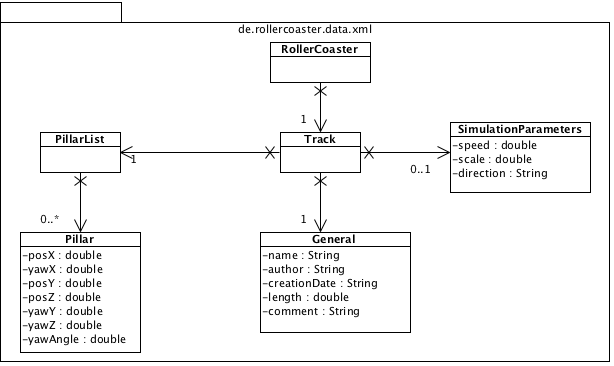
\includegraphics[width=\linewidth]{bilder/XML.png}
\caption{Deserialisiertes Schema für den Achterbahnsimulator}
\label{fig:xml}
\end{figure}

\section{Erläuterung}
Eine Achterbahn-Spezifikation wird durch \emph{RollerCoaster}
repräsentiert, die eigentliche Strecke \emph{Track}. Für jede Strecke
wird die Beschreibung in \emph{General}, die Angaben zur Simulation
in \emph{Simulation-Parameters} und die Liste der Stützstellen 
in \emph{PillarList} gespeichert. Aus den Stützstellen wird später eine
glatte Bahnkurve berechnet.

\section{XML-Schema}

\begin{verbatim}
<?xml version="1.0" encoding="utf-8"?>
<xs:schema id="RollerCoaster" targetNamespace="xml-schema-rollercoaster.xsd"
           elementFormDefault="qualified" attributeFormDefault="unqualified" 
           xmlns="xml-schema-rollercoaster.xsd" 
           xmlns:xs="http://www.w3.org/2001/XMLSchema">
  <xs:element name="RollerCoaster">
    <xs:complexType>
      <xs:sequence>
        <xs:element ref="Track" minOccurs="1" maxOccurs="1"/>
      </xs:sequence>
    </xs:complexType>
  </xs:element>
  <xs:element name="Track">
    <xs:complexType>
      <xs:sequence>
        <xs:element ref="General" minOccurs="1" maxOccurs="1"/>
        <xs:element ref="SimulationParameters" minOccurs="0" maxOccurs="1"/>
        <xs:element ref="PillarList" minOccurs="1" maxOccurs="1"/>
      </xs:sequence>
     </xs:complexType>
  </xs:element>
  <xs:element name="General">
    <xs:complexType>
      <xs:sequence>
           <xs:element name="Name" type="xs:string" minOccurs="1" maxOccurs="1"/>
           <xs:element name="Author" type="xs:string" minOccurs="1" maxOccurs="1"/>
           <xs:element name="CreationDate" type="xs:string" minOccurs="1" maxOccurs="1"/>
           <xs:element name="Length" type="xs:double" minOccurs="1" maxOccurs="1"/>
           <xs:element name="Comment" type="xs:string" minOccurs="1" maxOccurs="1"/>
      </xs:sequence>
    </xs:complexType>
  </xs:element>
   <xs:element name="SimulationParameters">
    <xs:complexType>
      <xs:sequence>
           <xs:element name="Speed" type="xs:double" minOccurs="1" maxOccurs="1"/>
           <xs:element name="Scale" type="xs:double" minOccurs="1" maxOccurs="1"/>
           <xs:element name="Direction" type="xs:string" minOccurs="1" maxOccurs="1"/>
      </xs:sequence>
    </xs:complexType>
  </xs:element>
  <xs:element name="PillarList">
    <xs:complexType>
      <xs:sequence>
        <xs:element ref="Pillar" minOccurs="0" maxOccurs="unbounded"/>
      </xs:sequence>
    </xs:complexType>
  </xs:element>
  <xs:element name="Pillar">
    <xs:complexType>
      <xs:sequence>
        <xs:element name="PosX" type="xs:double" minOccurs="1" maxOccurs="1"/>
        <xs:element name="PosY" type="xs:double" minOccurs="1" maxOccurs="1"/>
        <xs:element name="PosZ" type="xs:double" minOccurs="1" maxOccurs="1"/>
        <xs:element name="YawX" type="xs:double" minOccurs="1" maxOccurs="1"/>
        <xs:element name="YawY" type="xs:double" minOccurs="1" maxOccurs="1"/>
        <xs:element name="YawZ" type="xs:double" minOccurs="1" maxOccurs="1"/>
        <xs:element name="YawAngle" type="xs:double" minOccurs="1" maxOccurs="1"/>
      </xs:sequence>
    </xs:complexType>
  </xs:element>
</xs:schema>	
\end{verbatim}
